\documentclass[9pt]{beamer}
\usepackage[utf8]{inputenc}
\usepackage[russian]{babel}
\usepackage{graphicx, epsfig}
\usepackage{amsmath,mathrsfs,amsfonts,amssymb}
\usepackage{subfig}
\usepackage{floatflt}
\usepackage{epic,ecltree}
\usepackage{mathtext}
\usepackage{fancybox}
\usepackage{fancyhdr}
\usepackage{multirow}
\usepackage{enumerate}
\usepackage{epstopdf}
\usepackage{multicol}
\usepackage{algorithm}
\usepackage[noend]{algorithmic}
\def\algorithmicrequire{\textbf{Input:}}
\def\algorithmicensure{\textbf{Output:}}
\usetheme{Singapore}%{Singapore}%{Warsaw}%{Warsaw}%{Darmstadt}
\usecolortheme{default}
\setbeamertemplate{footline}[page number]{}
\newcommand{\bx}{\mathbf{x}}
\newcommand{\by}{\mathbf{y}}
\newcommand{\bz}{\mathbf{z}}
\newcommand{\bw}{\mathbf{w}}
\newcommand{\ba}{\mathbf{a}}
\newcommand{\bb}{\mathbf{b}}
\newcommand{\bY}{\mathbf{Y}}
\newcommand{\bX}{\mathbf{X}}
\newcommand{\bu}{\mathbf{u}}
\newcommand{\bt}{\mathbf{t}}
\newcommand{\bp}{\mathbf{p}}
\newcommand{\bq}{\mathbf{q}}
\newcommand{\bc}{\mathbf{c}}
\newcommand{\bP}{\mathbf{P}}
\newcommand{\bT}{\mathbf{T}}
\newcommand{\bB}{\mathbf{B}}
\newcommand{\bQ}{\mathbf{Q}}
\newcommand{\bC}{\mathbf{C}}
\newcommand{\bE}{\mathbf{E}}
\newcommand{\bF}{\mathbf{F}}
\newcommand{\bU}{\mathbf{U}}
\newcommand{\bW}{\mathbf{W}}
\newcommand{\bbR}{\mathbb{R}}
\newcommand{\cA}{\mathcal{A}}
\newcommand{\bchi}{\boldsymbol{\chi}}
\newcommand{\bnu}{\boldsymbol{\nu}}
\newcommand{\bmu}{\boldsymbol{\mu}}
\newcommand{\bOne}{\boldsymbol{1}}
\newcommand{\bZero}{\boldsymbol{0}}
\newcommand{\btheta}{\boldsymbol{\theta}}
\newcommand{\bTheta}{\boldsymbol{\Theta}}
\newcommand{\argmin}{\mathop{\arg \min}\limits}
\newcommand{\argmax}{\mathop{\arg \max}\limits}
\newcommand{\T}{\mathsf{T}}

\newcommand\undermat[2]{%
	\makebox[0pt][l]{$\smash{\underbrace{\phantom{%
					\begin{matrix}#2\end{matrix}}}_{\text{$#1$}}}$}#2}

\newtheorem{statement}{Утверждение}
\newtheorem{rustheorem}{Теорема}

% отображать название слайда слева
\setbeamertemplate{frametitle}[default][left]

\usepackage{tikz-cd}
%\definecolor{beamer@blendedblue}{RGB}{15,120,80}
%----------------------------------------------------------------------------------------------------------
\title[\hbox to 56mm{  \hfill\insertframenumber\,/\,\inserttotalframenumber}]
{\\ \vspace{1.5cm} Снижение размерности фазового пространства \\ в задачах канонического корреляционного анализа}
\author[Курдюкова Антонина]{\\ 
	\vspace{.4cm}
	Курдюкова Антонина\\
	\vspace{3mm}
	{\footnotesize Научный руководитель: \\
	д.ф.-м.н. В. В. Стрижов}}
\institute[МФТИ(НИУ)]{
Московский физико-технический институт\\
Факультет управления и прикладной математики\\
Кафедра <<Интеллектуальные системы>>}
\date{27 апреля 2022 г.}
%--------------------------------------------------------------------------------
\begin{document}
%--------------------------------------------------------------------------------
\begin{frame}
%\thispagestyle{empty}
\titlepage
\end{frame}
%--------------------------------------------------------------------------------
\begin{frame}{Снижение размерности фазового пространства}
	\begin{block}{Цель}
		Показать, что методы канонического корреляционного анализа являются частным случаем метода сходящихся перекрестных отображений Сугихары.
	\end{block}
	\begin{block}{Проблема}
		Сложная структура временного ряда -- наличие нелинейных зависимоей и варьирующийся период. \\
		Требуется построить адекватрную модель прогноза сигнала гироскопа для движения руки по сигналу акселерометра на этой руке.
	\end{block}
	\begin{block}{Решение}
		 Предлагается снизить размерность с использованием скрытого пространства и применить метод сходящихся перекрестных отображений для учёта причинно-следственных связей между рядами. 
	\end{block}
\end{frame}
%--------------------------------------------------------------------------------
\begin{frame}{Литература}
	\begin{itemize}
		\item De Brouwer E. et al. Latent convergent cross mapping //International Conference on Learning Representations. – 2020.
		\vfill
		\item Усманова К. Р. и др. Аппроксимация фазовой траектории квазипериодических сигналов методом сферической регрессии //Вестник Московского университета. Серия 15: Вычислительная математика и кибернетика. – 2020. – №. 4. – С. 40-46.
		\vfill
		\item Исаченко Р. В., Стрижов В. В. Снижение размерности с помощью проекции на скрытое пространство в задаче декодирования сигналов //Интеллектуализация обработки информации. – 2018. – С. 86-87.
		\vfill
		\item Sugihara G. et al. Detecting causality in complex ecosystems //science. – 2012. – Т. 338. – №. 6106. – С. 496-500.
		
	\end{itemize}
\end{frame}
%--------------------------------------------------------------------------------
\begin{frame}{Прогностическая модель}
	\begin{block}{Дано}
	\vspace{0.1cm}
	Выборка -- $\left( \bx, \by \right)$,\; где \quad
	$\bx = \{ x_1,\dots, x_{N_1}\}$,\quad
	$\by = \{ y_1,\dots, y_{N_2}\}$.\\
	\vspace{0.3cm}
	Требуется построить прогноз ряда $\bx$ на $m$ значений вперед:   \[x_{N_1 + 1},\dots, x_{N_1 + m}.\]
	При построение прогноза учесть влияние ряда $\by$ на $\bx$.
	\end{block}
\vspace{0.3cm}
\begin{block}{Модель}
    \vspace{0.1cm}
	При построении прогноза на один шаг вперед будем использовать $h$ предыдущих значений ряда $\bx$ и все предшествующие значения ряда $\by$:
	\[
		\hat{x}_{t+1} = \mathcal{F}(\hat{\bw}, x_t,\dots,x_{t-h+1}, y_t,\dots,y_1)
	\]
	\[
	    \hat{\bw} = \arg\min_{\bw} L(\bw, \bx, \hat{\bx})
	\]
	Здесь $L$~-- функция потерь.
	
\end{block}
	
\end{frame}
%--------------------------------------------------------------------------------
\begin{frame}{Снижение размерности пространства}
\begin{block}{Линейная зависимость}
\vspace{0.1cm}
	$\bX\in\bbR^{k\times n},\, \bY\in\bbR^{k\times r}$~-- матрицы фазовых пространств $\bx,\,\by$.\\
	Предполагается линейная зависимость между строками $\bX$ и $\bY$:
	\[
	    \mathbf{Y}_i = \mathbf{X}_i\cdot\mathbf{\Theta} + \boldsymbol{\varepsilon} \quad \mathbf{Y}_i\in\bbR^r,\;\mathbf{X}_i\in\bbR^n,\; i = 1,\ldots,k.
	\]
\end{block}
\vspace{-0.3cm}
\begin{block}{Метод частных наименьших квадратов (PLS)}
	\vspace{-0.5cm}
\begin{align*}
\underset{k \times n}{\vphantom{\bQ}\bX} 
&= \underset{k \times l}{\vphantom{\bQ}\bT} \cdot \underset{l \times n}{\vphantom{\bQ}\bP^{\T}} + \underset{k \times n}{\vphantom{\bQ}\bF} 
= \sum_{j=1}^l \underset{k \times 1}{\vphantom{\bp_j^{\T}}\bt_j} \cdot \underset{1 \times n}{\bp_j^{\T}} + \underset{k \times n}{\vphantom{\bp_j^{\T}}\bF},\\
\underset{k \times r}{\vphantom{\bQ}\bY} 
&= \underset{k \times l}{\vphantom{\bQ}\bU} \cdot \underset{l \times r}{\bQ^{\T}} + \underset{k \times r}{\vphantom{\bQ}\bE}
=  \sum_{j=1}^l  \underset{k \times 1}{\vphantom{\bq_j^{\T}}\bu_j} \cdot \underset{1 \times r}{\bq_j^{\T}} +  \underset{k\times r}{\vphantom{\bq_j^{\T}}\bE}.
\end{align*}
\end{block}
\vspace{-0.5cm}
\begin{block}{Ошибка}
	\vspace{-0.2cm}
\[
    L(\mathbf{\Theta}, \mathbf{X}, \mathbf{Y}) = \|\mathbf{Y} - \mathbf{X}\cdot\mathbf{\Theta}\|_2^2
\]
\vspace{-0.2cm}
\[
    \mathbf{\Theta} = \mathbf{W}(\mathbf{P}^{\mathsf{T}}\mathbf{W})^{-1}\mathbf{Q}^{\mathsf{T}}
\]
\end{block}

\end{frame}
%--------------------------------------------------------------------------------
\begin{frame}{Коммутативная диаграмма}
    \[
        \begin{tikzpicture}
			\matrix (m) [matrix of math nodes,row sep=3em,column sep=3em,minimum width=2em,ampersand replacement=\&]
			{
			    \& S \&
			    \\
				\mathbf{X}\in\bbR^{k\times n} \& \& \mathbf{Y}\in\bbR^{k\times r} \\
				\& \mathbf{T}, \mathbf{U} \in \bbR^{k\times\ell} \& \\};
			\path[-stealth]
			(m-1-2) edge [bend right=10] node {} (m-2-1)
			(m-1-2) edge [bend left=10] node {} (m-2-3)
			(m-2-1) edge node [above] {$\mathcal{F}$} (m-2-3)
			(m-2-1) edge [bend right=10] node [below, pos=0.4] {} (m-3-2)
			(m-3-2) edge [bend right=10] node [above, pos=0.4] {$\bP$} (m-2-1)
			(m-2-3) edge [bend left=10] node [below, pos=0.4] {} (m-3-2)
			(m-3-2) edge [bend left=10] node [above, pos=0.4] {$\bQ$} (m-2-3);
		\end{tikzpicture}
    \]
    
    \vspace{0.2cm}
    
    $S$~-- динамическая система,\\
    $\bX, \bY$~-- наблюдаемые фазовые пространства,\\
    $\bT,\bU$~-- латентно-согласованные пространства, не можем измерить.
\end{frame}
%--------------------------------------------------------------------------------
\begin{frame}{Метод Сугихары}
\begin{figure}[h]
\centering
\includegraphics[width = 250]{images_pr/attractor_new.jpg}
\end{figure}
\end{frame}
%--------------------------------------------------------------------------------
\begin{frame}{Метод перекрестных сходящихся отображений}
\begin{figure}[h]
\centering
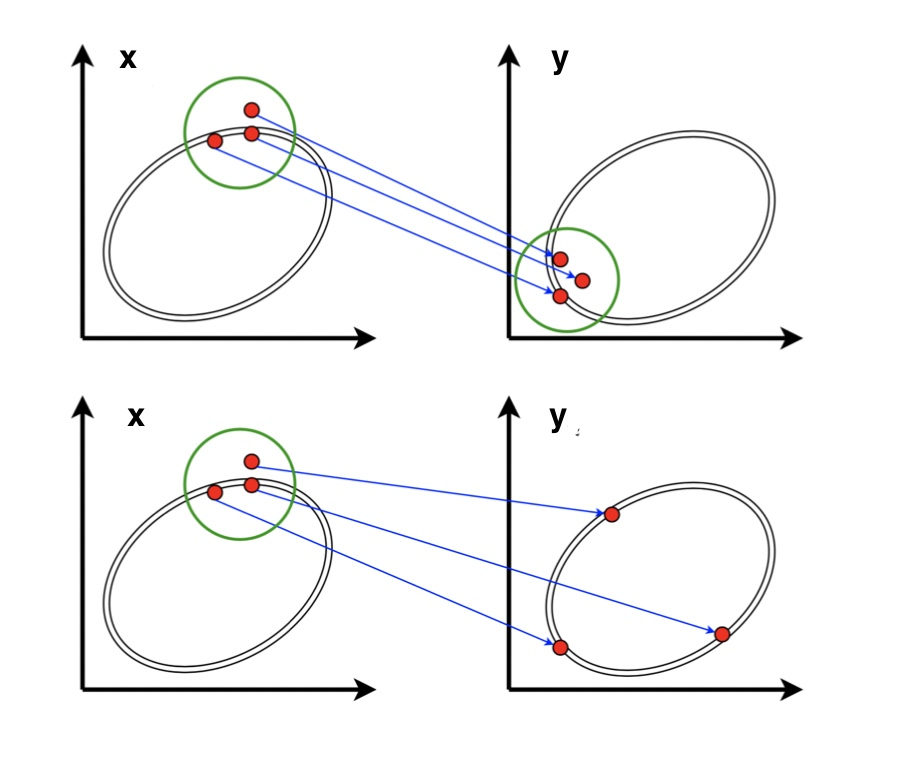
\includegraphics[width = 250]{images_pr/CCM.jpeg}
\end{figure}
\end{frame}
%--------------------------------------------------------------------------------
\begin{frame}{Вычислительный эксперимент}
\begin{block}{Данные}
\hfil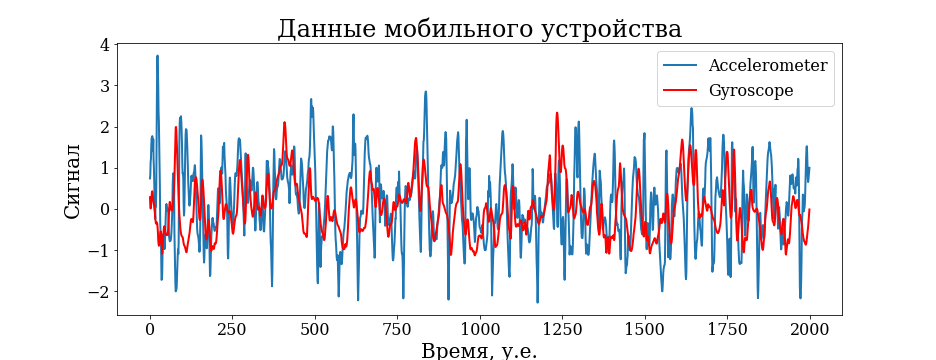
\includegraphics[width=6.5cm]{images_pr/signal.png}
\hfil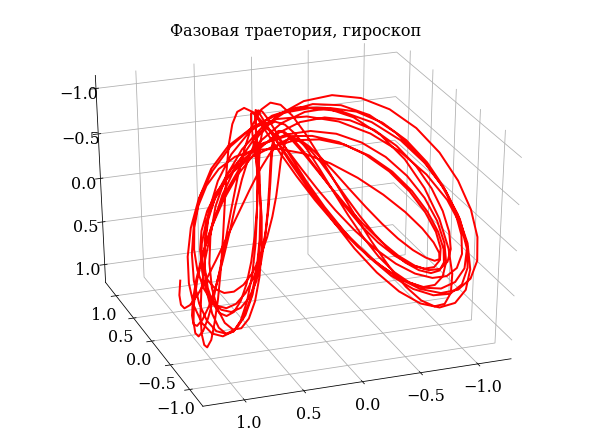
\includegraphics[width=4cm]{images_pr/gyr_tr.png}
\begin{itemize}
    \item Два телефона в одной руке
    \item Два телефона в заднем крмане
    \item Телефон в руке и в противоположном заднем кармене
\end{itemize}
\end{block}
\begin{block}{Цель}
	На примере решения прикладной задачи показать, что PLS -- частный случай метода Сугихары.\\
	Исследовать и другие методы, например Neural ODE.
\end{block}

\end{frame}
%--------------------------------------------------------------------------------
\begin{frame}{Заключение}
\begin{itemize}
	\item Показано, что методы канонического корреляционного анализа являются частным случаем метода Сугихары на примере PLS.
	\vfill
	\item Предложен метод обобщения PLS и CCM.
	\vfill
	\item Проведен вычислительный эксперимент на данных мобильного устройства.
	\vfill
	\item Показано, что учет зависимостей между временными рядами улучшает качество прогноза.
	\vfill
	\item Планируется рассмотреть другие методы канонического корреляционногот анализа.
\end{itemize}
\end{frame}
\end{document} 
